%%This is a very basic article template.
%%There is just one section and two subsections.
\documentclass[english,a4paper,numbers=noenddot]{article}

\usepackage{graphicx}
\usepackage{listings}
\usepackage{color}
\usepackage{amsmath}
\usepackage{makeidx}
\usepackage{hyperref}
\usepackage{parskip}
\usepackage{multirow}
\usepackage{tocloft}
\usepackage{textcomp}
\usepackage{wrapfig}

%\usepackage{times}
\renewcommand{\familydefault}{\sfdefault}

\renewcommand{\cftsecaftersnumb}{\hspace{6em}}
\renewcommand{\cftsubsecaftersnumb}{\hspace{6em}}
\renewcommand{\cftsubsubsecaftersnumb}{\hspace{6em}}

\makeindex

\hypersetup{
    %bookmarks=true,         % show bookmarks bar?
    unicode=false,          % non-Latin characters in Acrobats bookmarks
    pdftoolbar=true,        % show Acrobats toolbar?
    pdfmenubar=true,        % show Acrobats menu?
    pdffitwindow=false,     % window fit to page when opened
    pdfstartview={FitH},    % fits the width of the page to the window
    pdftitle={TDT4200 Parallel Computing - Problem Set 4 - hvatum},    % title
    pdfauthor={Stian Hvatum},     % author
    pdfsubject={TDT4200 Parallel Computing},   % subject of the document
    pdfcreator={Stian Hvatum},   % creator of the document
    pdfproducer={Stian Hvatum}, % producer of the document
    pdfnewwindow=true,      % links in new window
    colorlinks,       % false: boxed links; true: colored links
    linkcolor=black,          % color of internal links
    citecolor=green,        % color of links to bibliography
    filecolor=magenta,      % color of file links
    urlcolor=cyan           % color of external links
}

\definecolor{listinggray}{gray}{0.9}
\definecolor{lbcolor}{rgb}{0.9,0.9,0.9}
\lstset{
    keywordstyle=\bfseries\ttfamily\color[rgb]{0,0,1},
    identifierstyle=\ttfamily,
    commentstyle=\color[rgb]{0.133,0.545,0.133},
    stringstyle=\ttfamily\color[rgb]{0.627,0.126,0.941},
    showstringspaces=false,
    basicstyle=\tiny,
    numberstyle=\tiny,
    framexleftmargin=3pt,
    numbers=left,
    stepnumber=1,
    numbersep=15pt,
    tabsize=2,
    breaklines=true,
    prebreak = \raisebox{0ex}[0ex][0ex]{\ensuremath{\hookleftarrow}},
    breakatwhitespace=false,
    aboveskip={1.5\baselineskip},
    columns=fixed,
    upquote=true,
    extendedchars=true,
  	frame=l,
    sensitive=true,
}

\renewcommand{\thesection}{Task \arabic{section}}
\renewcommand{\thesubsection}{\arabic{subsection}.}
\renewcommand{\thesubsubsection}{\alph{subsection}) \arabic{subsubsection}.}

\title{TDT4200 Parallel Computing\\
\Huge Problem Set 4}
\author{Stian Hvatum (hvatum)\\MTDT}

\begin{document}
\maketitle
\tableofcontents
\newpage
\section{Theory}
\subsection{Differences between processes and threads}
\begin{enumerate}
    \item Processes have their own private virtual memory space provided by the operating system, while threads within one process share this memory space among each other.\hfill
    \item Processes do not usually share resources with each other, while threads within one process usually share the allocated resources.\hfill
    \item Processes are usually scheduled by the operating system, while thread scheduling is much more controlled by the programmer\footnote{Still, threads are usually preemptive scheduled by the OS, but the programmer can sleep, wake, create and join threads as he wants}.\hfill
\end{enumerate}

\subsection{OpenMP vs. POSIX Threads}
\subsubsection{Benefits of OpenMP}
OpenMP code is generally more readable than POSIX Thread programs. OpenMP is also much easier to use when you parallelize an already existing serial program, since you add almost only pragmas instead of having to rewrite the entire program.

\subsubsection{Benefits of POSIX Threads}
POSIX Threads and the pthreads library gives the programmer much more fine grained control of the threads than OpenMP, while you still can get equal speed as OpenMP. pthreads is also in my opinion easier to use when you have a real world application that do different things at the same time, eg. listening for incoming network traffic while prompting the user for input.

\subsection{Mutex vs. Semaphore}
Mutexes and semaphores are both utilities for synchronization in parallel programs. A mutex is a kind of lock, such that one thread can only acquire the lock if no one else has acquired it. Once a lock is required, it must be released by it's owner before someone else can lock it. This provides us with a method to allow only one thread through a critical section at a time. The first thread will acquire lock on the mutex, while later threads will wait at the lock(mutex)-call until the owner unlocks it. Then, one of the waiters will acquire lock, and passes by, while the remaining threads still wait for their turn. Similar to mutexes, semaphores also provides this kind of mechanism, but semaphores uses a kind of resource counter to allow a certain number of threads/calls to pass through.

A common example for using semaphores are the producer/consumer-pattern, where two semaphores represents number of produces elements and number of empty spaces to put produced elements in. At each production, the produced counter is incremented, and the number of spaces are decremented. When there are no more spaces left, the producer will go to sleep until the semaphore in incremented by the consumer. The consumer increments the number of empty spaces and decrements the number of produces elements at each "consume", and goes to sleep if number of produces elements is zero.

A good example of using mutexes is programs that contains critical sections, eg. global variable updating, and needs to ensure that only one thread at a time updates the variable. If this global variable is updated multiple places in the same program, we can use the same mutex on the different locations to ensure that only one thread are running in only one of the locations.

\subsection{Reduction}
When we are updating a number in parallel, we may run into a race condition. If we are using the same arithmetic operation in each thread, we can divide the problem such that each thread calculates their part, and then we group threads, eg. into a binary tree, and pass the resulting parts against the root. In this way, we get $log_2(N)$ arithmetic operations that has to be synchronized instead of N operations. One possible implementation is illustrated in Figure \ref{pr}.
\begin{figure}
    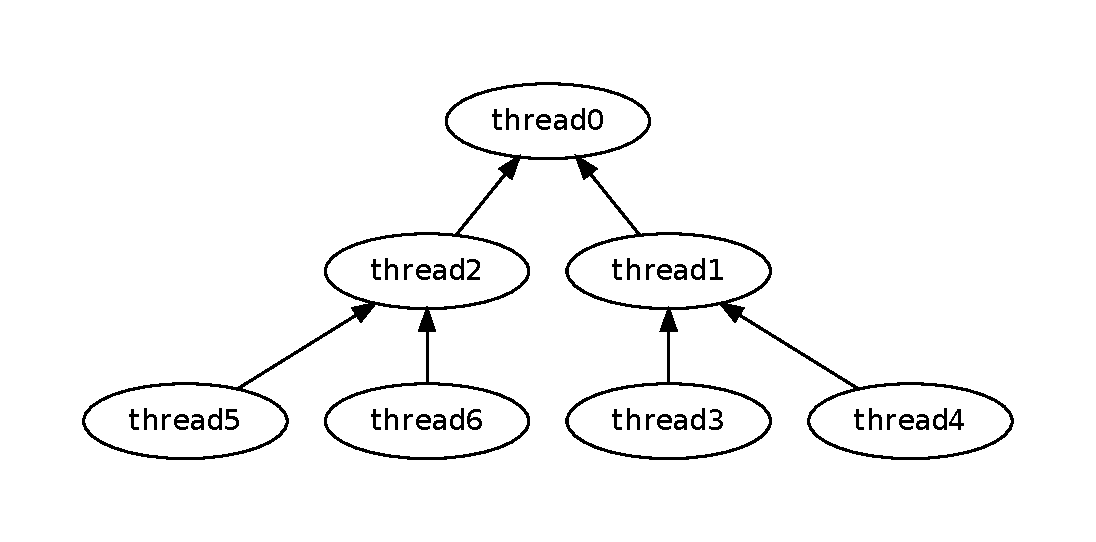
\includegraphics{reduction.pdf}
    \caption{Passing results}
    \label{pr}
\end{figure}

\subsection{Race condition}
The code in Figure \ref{rc} is a simple program that adds all numbers from 0 to 9 (excluding 10). The code is really simple, but the inclusion of OpenMP generates a severe problem. When we parallelize the loop, multiple threads will read \texttt{sum}, add \texttt{i} to it, and store the value back into \texttt{sum}. Since threads often are interleaved, one thread may write back \texttt{sum} right after another thread has read it, but before it has added to it. If this happens, the last thread will overwrite \texttt{sum} with a sum that skipped the other thread's addition. This phenomenon is called a race condition since the threads "races" to gain access to a resource.
\begin{figure}[caption={Race condition},captionpos=b]
    \lstinputlisting[language=C]{racecond.c}
    \caption{Race condition}
    \label{rc}
\end{figure}

\subsection{Thread safety}
If a function is \textit{thread-safe}, it can safely be used in a multithreaded program. When a function is \textit{thread-safe}, it basically means that multiple threads will not get in each others way if they call the function simultaneously. If all modified variables are one the current threads stack, or they are locked in a proper way, a function will in most cases be thread safe\footnote{Given they don't call any thread-unsafe functions}. 

The \texttt{fibonacci}-function can not be considered \textit{thread-safe}. The reason is that it makes use of \texttt{static} variables, which are not completely local. A static variable is a "local" variable that is stored somewhere else than on the stack\footnote{There is no standard place for static variables, but GCC tends to store it at .bss (Block Started by Symbol)}. Since it is not stored on the stack, it's value is kept between calls, and subsequent calls can continue where the last stopped, like in the \texttt{fibonacci}-function.

These static variables creates a problem for multithreaded programs, since if an other thread calls the function while a first thread is in the middle of it, the new thread will alter the value of the static variable, and suddenly both threads call the function within the same "state". This is the same as for global variables, and can not be considered thread safe.

\section{Programming}
\subsection{OpenMP}
See nbody\_openmp.c
\subsection{POSIX threads}
See nbody\_pthreads.c
\subsection{Speedup}
I have tested both programs against the serial program on clustis3.idi.ntnu.no, and the speedup was as shown in Table \ref{speedup}. I receive almost linear speedup in the OpenMP-version, this is probably because the most computational-heavy parts of the program has been parallelized. In the pthreads-version, everything is block-scheduled among the threads, which may bad for cache if threads are evenly interleaved. On my personal computer\footnote{Intel i7 930 @ 2.8GHz}, the difference where much less, though the wall clock time for 9 threads\footnote{On 8 threads, OpenMP used 2.3 seconds!} for both where about 0.360 seconds, OpenMP being slightly faster. The number of planets in the test where 1002, as in the provided planets.txt-file. If I use some more than 8 threads, the speedup for both are minimal, since this is the number of cores (including HT) on both my private computer and clustis. If I use fewer time steps, pthreads seems to be faster, while more time steps seems to boost OpenMP. I believe this is because pthreads can schedule the work with less overhead, and thus use less work on getting started, while OpenMP have better scheduling of threads, and have better throughput once started.

\begin{table}
    The Serial, pthreads and OpenMP-values are wall clock time for running the program with 100 time steps, \# threads and 1002 planets. The speedup-columns are the running time of the serial program devided by the running time of the parallelized program in the left-of column.
    \begin{tabular}{|c|c|c|c|c|c|}
        \hline
        %%%%%%%%%%%%%%%%%%%%%%%%%%%%%%%%%%%%%%%%%%%%%%%%%%%%%%%%%%%%%%%%%%%%%%
%%                                                                  %%
%%  This is a LaTeX2e table fragment exported from Gnumeric.        %%
%%                                                                  %%
%%%%%%%%%%%%%%%%%%%%%%%%%%%%%%%%%%%%%%%%%%%%%%%%%%%%%%%%%%%%%%%%%%%%%%
\# threads	&Serial	&pthreads	&Speedup	&OpenMP	&Speedup\\
\hline
1	&1.034	&1.107	&0.934	&1.036	&0.998\\
2	&1.034	&0.843	&1.227	&0.535	&1.933\\
3	&1.035	&0.632	&1.638	&0.363	&2.851\\
4	&1.035	&0.504	&2.054	&0.278	&3.723\\
5	&1.035	&0.427	&2.424	&0.225	&4.600\\
6	&1.035	&0.365	&2.836	&0.202	&5.124\\
7	&1.034	&0.328	&3.152	&0.170	&6.082\\
8	&1.034	&0.293	&3.529	&0.154	&6.714\\

        \hline
    \end{tabular}
    \caption{Speedup}
    \label{speedup}
\end{table}
\end{document}
